\documentclass{standalone}
\usepackage{amsmath}
\usepackage[compat=1.1.0]{tikz-feynman}

\definecolor{MyBlue}{RGB}{0, 68, 136}
\definecolor{MyYellow}{RGB}{221, 170, 51}
\newcommand{\lw}{0.8pt}

\begin{document}
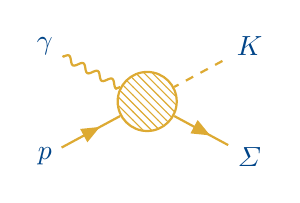
\begin{tikzpicture}[every edge/.append style={line width=\lw}]
  \begin{feynman}
    \vertex[text=MyBlue] (g)   at (-1.3,  0.7) {$\gamma$};
    \vertex[text=MyBlue] (p)   at (-1.3, -0.7) {$p$};
    \vertex[text=MyBlue] (ks)  at ( 1.3,  0.7) {$K$};
    \vertex[text=MyBlue] (sig) at ( 1.3, -0.7) {$\varSigma$};
    \vertex[blob, draw=MyYellow, line width=\lw, pattern color=MyYellow] (C) at (0,0) {};
    \diagram*{
    (g)  -- [photon, color=MyYellow] (C),
    (p)  -- [fermion, color=MyYellow] (C),
    (C)  -- [fermion, color=MyYellow] (sig),
    (C)  -- [scalar, color=MyYellow, dash phase=1.2pt] (ks),
    };
  \end{feynman}
\end{tikzpicture}
\end{document}
